\documentclass[a4paper, punct,space,fancyhdr, fntef,UTF8]{ctexart}


\usepackage{szutils}%在这里放置需要的宏包,并设置部分所需内容
\usepackage{romannum}
\usepackage{zhlipsum}
\setcounter{secnumdepth}{4}

\begin{document}

	\pagestyle{empty}%不要页眉页脚
	%封面与诚信声明
	
%\centerline{\kaishu\zihao{-0}{深圳大学}}
\begin{figure}[htbp]
	\begin{center}
		
\includegraphics[width=2.7in]{szu}
	\end{center}
\end{figure}


\centerline{\heiti\zihao{1}{本\ 科\  毕\  业\  论\  文\  (设计)}}

\vskip 3.5cm



\begin{flushleft}
	\zihao{3}
	\hspace{3cm}{\heiti{题目:}}      
	{\kaishu\underline{\quad\textbf{智能网联汽车GNSS位置欺骗攻击与功能}}}
	\vspace{10bp}
	\hspace{3cm}{\kaishu\underline{\hspace{2.7cm}\quad\textbf{安全危害联动预警策略设计及实现}\hspace{2.1cm}}}
	% \vspace{10bp}
	
	\hspace{3cm}{\heiti{姓名:}}      
	{\kaishu\underline{\hspace{2.8cm}\textbf{李宇良}\hspace{3.5cm}}}              \\
	\vspace{10bp}
	
	\hspace{3cm}{\heiti{专业:}}     
	{\kaishu\underline{\hspace{1.5cm}\textbf{计算机科学与技术}\hspace{2cm}}}            \\
	\vspace{10bp}
	
	\hspace{3cm}{\heiti{学院:}}      {\kaishu\underline{\hspace{1.5cm}\textbf{计算机与软件学院}\hspace{2cm}}}               \\
	\vspace{10bp}
	
	\hspace{3cm}{\heiti{学号:}}      {\kaishu\underline{\hspace{2.4cm}\textbf{2018151004}\hspace{2.6cm}}}                   \\
	\vspace{10bp}
	
	\hspace{3cm}{\heiti{指导教师:}} 
	{\kaishu\underline{\hspace{1.8cm}\textbf{肖志娇}\hspace{3.5cm}} }                         \\
	\vspace{10bp}
	
	\hspace{3cm}{\heiti{职称:}}      
	{\kaishu\underline{\hspace{3.2cm}\textbf{副教授}\hspace{3.8cm}} }                         \\
	
\end{flushleft}

\vskip 4cm

\centerline{\zihao{3} 2022 年 \  4 月\  1 日}
	\newpage

\centerline{\heiti\zihao{-2}{深圳大学本科毕业论文(设计)诚信声明}}


\vskip 3cm 


\begin{spacing}{2.0}
	\zihao{4}
本人郑重声明:所呈交的毕业论文(设计),题目《智能网联汽车GNSS位置欺骗攻击与功能安全危害联动预警
策略设计及实现》是本人在指导教师的指导下,独立进行研究工作所取得的成果。对本文的研究做出重要贡献的个人和集体,均已在文中以明确方式注明。除此之外,本论文不包含任何其他个人或集体已经发表或撰写过的作品成果。本人完全意识到本声明的法律结果。

\vskip 3cm

{\flushright{
		毕业论文(设计)作者签名:\hspace{2.2cm}
		
		
		
		\hspace{7.5cm}{日期:\hspace{2cm}年 \hspace{.5cm}月\hspace{.5cm}日}\hspace{4cm} 
	}}
\end{spacing}





	\zihao{-4}
	\tableofcontents%生成目录
	\thispagestyle{empty}%页脚不要页码
	%“目录”两个字的样式与section的样式一致,默认居中,故将设置section标题居左放置在生成目录后
	\ctexset{section={format=\Large\bfseries}}  %section标题居左

	%%%%正文开始,页脚有页码
	\cfoot{\zihao{-5}第 \ \thepage \ 页 \ 共 \ \pageref{lastpage} 页}%%%%lastpage为末页标签
	%正文
	\zihao{5}
	\pagenumbering{arabic}%页码使用阿拉伯数字
	\setcounter{page}{0}  %重新设置页码计数
	\pagestyle{fancy}

	\newpage


\centerline{\fangsong\bf\zihao{-2}{智能网联汽车GNSS位置欺骗攻击}}
\vspace{\baselineskip}
\centerline{\fangsong\bf\zihao{-2}{与功能安全危害联动预警策略设计及实现}}
\addcontentsline{toc}{section}{摘要(关键词)}%加入目录


\vskip 1cm

\begin{center}
	\kaishu
	\hspace{2cm}计算机与软件学院计算机科学与技术专业 \quad 李宇良 
	\vspace{5bp}
	\newline
	学号:2018151004
\end{center}

\vskip 10bp

{
\kaishu	
\hspace{5bp}{\zihao{-4}\textbf{【摘要】}} 
\zhlipsum

\vskip 10bp

\hspace{5bp} {\zihao{-4}\textbf{【 关键词】}} 
推荐系统; 协同过滤; 适应性采样  
}
    \section{引言}

\subsection{研究背景及意义}
近年来,随着现代通信技术以及自动驾驶技术的迅速发展,汽车这一传统出行载体也在往智能化、互联化的发展方向迈进。由此诞生出来的新产物便是智能网联汽车。区别于一般的自动驾驶汽车(ADAS),智能网联汽车可以理解为在自动驾驶技术的基础上(即自动驾驶决策单元、对应的传感器、控制器等),将车联网技术融合其中,使得汽车可以与周围环境、道路、甚至“云”,进行信息的沟通与共享,从而实现V2X(Vehicle to X)[智能网联汽车信息安全威胁识别和防护方法研究-郝晶晶]。这种互联化的技术可以使得传统自动驾驶汽车拥有更全面复杂的环境感知能力与决策能力,从而提高自动驾驶汽车的安全性与可靠性,并最终实现可以替代驾驶员所有操作的“无人驾驶汽车”。

外部网络接入带来的不仅有自动驾驶汽车各项能力的提升,随之而来的还有针对智能网联汽车的信息安全威胁。据国家工信部统计,自2020年以来,针对车联网信息服务提供商、整车企业等相关企业的恶意攻击高达280万起[引用白皮书];另外,截止到2020年底,全球范围内共发现110个与汽车产品相关的CVE漏洞。这些漏洞涉及范围广泛,包含汽车的内部网络、网关、传感器、车载信息娱乐系统、蓝牙、OBD端口等等部件。这些针对汽车产品的安全漏洞以及攻击不仅会影响用户的信息娱乐服务质量,威胁用户的信息安全,甚至还很有可能导致汽车控制功能失效,直接威胁车内乘客的人身安全。由此可见,智能网联汽车相关的信息安全问题亟待解决。

一般而言,与智能网联汽车相关联的信息风险可以分为IP流量攻击风险,CAN流量攻击风险,GNSS位置欺骗攻击,蓝牙攻击风险以及车机攻击风险[这里引用一个文章]。本文主要关注GNSS位置欺骗攻击,其中包括攻击检测以及对应功能安全危害的预警策略。

GNSS位置欺骗攻击最早出现在军事领域。2011年12月,伊朗使用GNSS位置欺骗攻击技术,成功控制了美军的RQ-170“哨兵”无人机,使其降落到伊朗机场。2016年1月,美国海军的两艘小型巡逻艇在执行任务时偏离原本的航行路线,进入了伊朗海域,从而使船只与美国军方失去联系。而在民用领域,2014年3月,从吉隆坡国际机场飞往北京首都机场的MH370航班在航行过程中失联,迄今尚未发现任何残骸。一些专家认为,MH370很可能受到欺骗性的干扰,导致其偏离航线并在耗尽燃料后坠毁。从技术角度来看,GNSS位置欺骗攻击确实具有这种潜在的攻击力\cite{bian2017research}。近十年来,随着对该类攻击的深入研究,学术界已经有多种相对成熟的攻击检测方法。然而,这些研究大多数集中在军事领域,而由于军事设施与汽车在GNSS设备条件上的差异,这些成果往往不能直接应用到智能网联汽车上。而目前少部分聚焦于智能网联汽车GNSS位置欺骗研究的工作,往往仅关心GNSS位置欺骗攻击的检测方法,而忽略了攻击发生后可能会对汽车带来的功能安全危害,以及在攻击已经无法挽回的情况下如何采取应急策略来最小化损失。本文针对上述背景,提出了一种可以用于智能网联汽车GNSS位置欺骗攻击的检测方法,并在此基础上,提出相应的功能安全联动预警与应急策略,构建一个完整的“检测-预警-应急”系统。

\subsection{本文主要工作}
本论文分为六章,内容分别如下:

第一章为引言,主要介绍本论文的研究背景、研究意义、主要工作以及论文的组织结构。

第二章为相关技术简介,主要介绍与本论文工作相关的基础技术细节,包括GNSS原理概述,LSTM原理概述,汽车功能安全以及国内外对本文工作的研究现状。

第三章为基于LSTM进行汽车位置预测的GNSS位置攻击欺骗检测模型,介绍了如何基于LSTM构建一个可用于智能网联汽车的GNSS位置欺骗攻击检测算法。

第四章为GNSS位置欺骗攻击功能安全应急策略,主要介绍应对GNSS位置欺骗攻击的功能安全应急策略,以及如何将检测算法与应急策略进行联动。

第五章为实验与结果分析,主要介绍基于CARLA模拟器的仿真实验细节,以及具体的实验结果与分析。

第六章为结论与展望,主要是简要总结本文工作,并对进一步的研究工作提出展望。

\subsection{本文贡献}

	\section{相关技术简介}

\subsection{GNSS(全球卫星导航系统)概述}
全球卫星导航系统(Global Navigation Satellite System,下称GNSS),一般是指通过覆盖全球的导航卫星系统为地面或近地面用户提供全天候的三维空间坐标以及时间信息的无线定位系统。使用GNSS进行定位的用户可以通过具有GNSS信号接收器接收来自当前区域卫星的定位信号,并通过一系列的解码与计算得到较为准确的空间信息与时间信息,从而实现定位、导航、授时(PNT)的功能。

世界上第一个全球卫星导航系统是美国的GPS系统。该系统在设计之处一共由24颗卫星组成,其中21颗为工作卫星,3颗为备用卫星。而截至到目前,GPS系统的卫星数目已经达到了31颗。而在我国,第一颗北斗卫星在2007年4月14日发射,被在往后的若干年里不断完善北斗导航系统。截至2020年,北斗系统已经实现向全球提供服务的目标,与美国GPS、俄罗斯GLONASS、欧盟GALILEO并列成为四大全球定位系统。除了上述的全球性定位系统外,还包括区域系统和增强系统。其中区域系统有日本的QZSS和印度的IRNSS;增强系统则包括美国的WASS、日本的MSAS以及欧盟的EGNOS等。

GNSS的定位原理可以认为是求解一组方程。对于用户所处空间位置$(x_u, y_u, z_u)$,由于导航卫星所处的精确位置是可知的,同时卫星与用户之间的距离也可通过光速与时间差得到,因此可以列出以下方程组。
\begin{equation}
    \begin{cases}
        \rho_1=\sqrt{(x_1-x_u)^2+(y_1-y_u)^2+(z_1-z_u)^2}\\
        \rho_2=\sqrt{(x_2-x_u)^2+(y_2-y_u)^2+(z_2-z_u)^2}\\
        \rho_3=\sqrt{(x_3-x_u)^2+(y_3-y_u)^2+(z_3-z_u)^2}\\
    \end{cases}
    \label{eq:1}
\end{equation}
其中,$x_i$,$y_i$,$z_i$表示当前用于定位用户位置的第$i$颗卫星的空间位置。$\rho_i$则表示用户距离第$i$颗卫星的距离。求解上述方程组,即可求得用户位置坐标$(x_u,y_u,z_u)$。然而,在实际应用中,除了上述的三个未知数以外,往往还需要第四个未知数$t_u$作为修正项。原因在于,在计算用户位置与卫星间距离时,需要使用导航卫星中的原子钟与地面用户接收器的时钟作差得到钟差,但接收器的时钟精度要比原子钟精度低。这就导致最终得到的钟差会有一定的误差,因此需要加入修正项。此时的方程组为。
\begin{equation}
    \begin{cases}
        \rho_1=\sqrt{(x_1-x_u)^2+(y_1-y_u)^2+(z_1-z_u)^2}+ct_u\\
        \rho_2=\sqrt{(x_2-x_u)^2+(y_2-y_u)^2+(z_2-z_u)^2}+ct_u\\
        \rho_3=\sqrt{(x_3-x_u)^2+(y_3-y_u)^2+(z_3-z_u)^2}+ct_u\\
        \rho_4=\sqrt{(x_4-x_u)^2+(y_4-y_u)^2+(z_4-z_u)^2}+ct_u\\
    \end{cases}
    \label{eq:2}
\end{equation}
其中,$c$表示光速。
\subsection{GNSS位置欺骗攻击及检测方法概述}
目前,GNSS位置欺骗攻击还没有精确的定义。一般而言,“欺骗”是指某人或某程序利用数据篡改、数据伪造等手段成功伪装成另一个人或另一个程序,其目的往往是获取情报或影响被攻击者的正常运作。具体到GNSS位置欺骗攻击方面,攻击者会通过伪造错误定位信号或转发真实卫星信号等手段进行攻击。遭受欺骗攻击的GNSS接收器则会计算出一个错误的位置或错误的时间,从而导致依赖于GNSS定位的其他部件工作受阻或出错,甚至是无法工作。下面将对常见的GNSS位置欺骗攻击手段及检测方法进行简要介绍。
\subsubsection{欺骗方法概述}
\paragraph{基于信号模拟器的自主产生式攻击}

该攻击方式的主要思想是通过一个GNSS信号模拟器发送虚假GNSS定位信号来实现欺骗目的。目前,诸如Spirent公司的GSS8000等GNSS信号模拟器可以模拟出各种真实环境中的卫星定位信号。通过向接收机发送生成的定位信号的方法,可以实现一定程度上的位置欺骗攻击。但这种方法的缺点也很明显。由于GNSS信号模拟器所产生的信号是完全自主产生的,并没有与实际卫星进行信号同步,所以很容易导致接收机出现失锁或重捕的问题,从而导致欺骗被检测。另外,GNSS模拟器庞大的体积以及高昂的价格也是该欺骗方法的主要缺点之一。
\paragraph{基于接收机的接受产生式攻击}

该攻击方式所使用的干扰源主要由两部分组成,即接收机与信号模拟器。接受产生式攻击的基本工作原理与自主产生式攻击类似,都需要使用一个信号模拟器进行信号模拟生产。两者最大的不同在于,前者在产生虚假定位信号时所使用的参数由操作者或机器自身自主设置;而后者则是根据接收机接收到的真是卫星信号的估计结果,通过算法计算得到。与自主产生式攻击相比,接收产生式攻击所产生的信号与真实信号接近,其隐蔽性要更强。而其缺点在于,由于在使用真实卫星信号计算模拟参数时需要精确测定目标接收机与欺骗干扰源之间的三维位置关系,实现难度较大。尤其是当欺骗目标处于运动状态的时候,需要实时测定两者位置关系。也正因如此,这种欺骗手段一般只用于静止状态或低速运动状态下的目标。
\paragraph{基于信号转发器的转发式攻击}
\label{par:zhuanfa}

我国在GNSS欺骗方面的研究主要集中在转发式攻击。该攻击手段所采用的思路与上述两种欺骗方法截然不同。该方法不再生成虚假信号,而是直接使用真实的卫星导航信号,通过使用转发器发射到目标区域,从而使目标接收到另一个空间位置的GNSS定位信号。与产生式攻击方法相比,该方法最大的优点在于不需要了解信号的内部细节(如GNSS信号格式、加密方式等),从而避免了大量技术细节与限制,并因此扩大了适用范围。而该方法的最大缺点在于,由于在信号转发时需要对原始信号放大,这会导致信号中的噪声被一起放大,从而导致转发信号与接收机接收到的真实定位信号在噪声水平上有较大的差别,容易被检测到。
\subsubsection{检测方法概述}
\paragraph{基于空间信息处理的检测方法}

该检测方法的主要思想是通过判别导航信号的空间信息来实现欺骗检测。具体来说,GNSS在定位时会从不同方向的不同卫星向用户发送定位信号;而欺骗源往往是从同一方向发射多个信号。通过处理接收到的信号,解算出信号的大致空间特征,就可以识别出当前收到的信号是否为欺骗信号。由于卫星的空间信息几乎是不可能被模仿的,因此这种检测方法是目前最为有效的GNSS欺骗检测方法之一。
\paragraph{基于信号到达时间的检测方法}

该检测方法的主要思想是通过判断欺骗信号与真实信号在到达时间上的差异来实现欺骗检测,主要用于转发式攻击。从\ref{par:zhuanfa}中可以看出,当使用欺骗设备对真实信号进行接收并转发后,目标接收机所接收到的信号必然会与真实信号在时间上有一定的延迟。根据这一特征,便可以判断当前是否收到了欺骗攻击。与转发式欺骗攻击方法一样,这种检测方法也是更适用于固定位置的接收机,在动态场景下的适用性有待提高。

\paragraph{基于机器学习的检测方法}
机器学习的方法也被应用到GNSS欺骗攻击检测中。举例而言,Semanjski S等人\cite{semanjski2020gnss}将欺骗检测问题转化为分类问题,并使用SVM的方法来区分真实信号与欺骗信号,从而实现检测目的。L.Junzhi等\cite{Junzhi2019gan}探讨了使用生成对抗网络(GAN)来进行GNSS欺骗检测的可行性;Dasgupta等人\cite{dasgupta2021reinforcement}将强化学习(Reinforcement Learning)的方法应用到GNSS的欺骗攻击检测中,通过使用来自自动驾驶汽车的GNSS定位信息、加速度、速度以及方向盘转向角,构建出一个可实现实时(turn-by-turn)欺骗检测的强化学习模型。


\subsection{LSTM概述}

\begin{equation}
    f_i^{(t)}=\sigma\bigg(b_i^f+\sum_jU_{i,j}^fx_j^(t)+\sum_jW_{i,j}^fh_j^{(t-1)}\bigg)
    \label{eq:3}
\end{equation}

\begin{equation}
    s_i^{(t)}=f_i^{(t)}s_i^{(t-1)}+g_i^{(t)}\sigma\bigg(b_i+\sum_jU_{i,j}x_j^{(t)}+\sum_jW_{i,j}h_j^{(t-1)}\bigg)
    \label{eq:4}
\end{equation}

\begin{equation}
    g_i^{(t)}=\sigma\bigg(b_i^g+\sum_jU_{i,j}^gx_j^{(t)}+\sum_jW_{i,j}^gh_j^{(t-1)}\bigg)
    \label{eq:5}
\end{equation}

\subsection{汽车功能安全概述}
\subsection{国内外研究现状}
\subsubsection{智能网联汽车GNSS位置欺骗攻击检测方面}
\subsubsection{基于预测的GNSS位置欺骗攻击检测算法}
\subsubsection{智能网联汽车GNSS功能安全方面}
\subsection{本章小结}

	\section{预备知识}

\subsection{Bayesian Personalized Ranking}
\begin{figure}[htbp]
	% caption放上面就会显示在图的上方,出现在下面就是出现在图的下方
	% label的位置也有讲究
	\begin{center}
		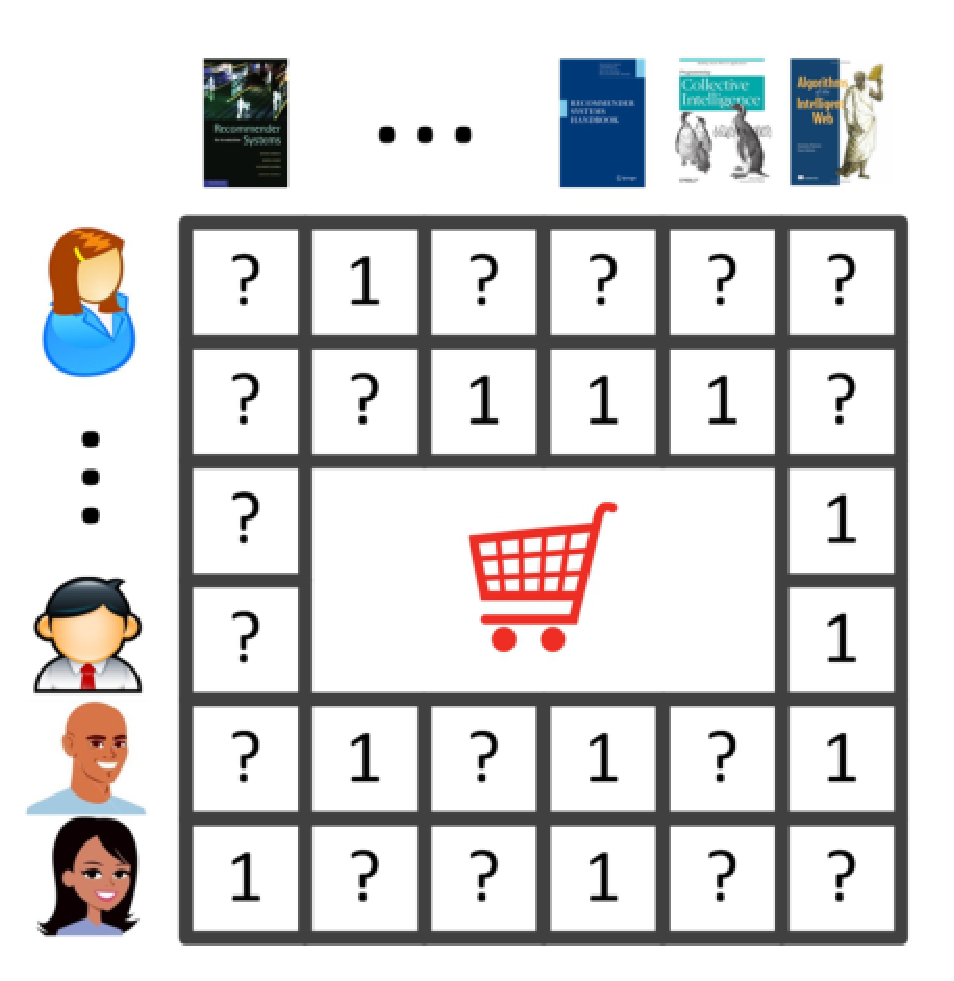
\includegraphics[width=3in]{matrix}
		\caption{user-item 隐式反馈矩阵}
		\label{gra3}
	\end{center}
\end{figure}
在这一节, 我们首先回顾BPR算法,然后讨论它的一些局限性,也就是其收敛缓慢与冷启动问题。通常用户与物品的隐式反馈可以表示为如图\ref{gra3}所示的矩阵, 矩阵的“1”表示用户已经对该物品有过交互行为, 比如购买,点击等, 矩阵的“?”则表示用户还未对该物品有过交互行为。

\subsubsection{Pairwise Preference Assumption}
BPR\cite{rendle2009bpr}是一个应对隐式反馈很流行的推荐框架. 它基于这样一个偏好假设: 如果一个用户$u$已经选择了物品$i$但是没有选择物品$j$,那么在BPR中, 我们认为相对于物品$j$用户$m$更喜欢物品$i$,并定义用户$u$关于物品$i$与$j$的偏好关系为:
\begin{equation}
\label{pairwisepre}
p \left( i \succ_u j \right) := f \left( x_{uij} \right),
\end{equation}
这里$f \left(x\right) = 1/\left(1+exp\left(-x\right)\right)$\footnote{$f \left(x\right)$即为sigmoid函数}, $x_{uij} := s\left(u,i\right) - s\left(u,j\right)$, $s\left(\cdot,\cdot\right)$可以是任何表示用户与物品相关程度的函数。在BPR\cite{rendle2009bpr}中, $s\left(\cdot,\cdot\right)$为用户对物品的预测值, 即$s\left(u,i\right) = \hat{r}_{ui}$, $x_{uij} = \hat{r}_{ui}-\hat{r}_{uj}$.


\subsubsection{预测公式}

在BPR中, 用户$u$对于物品$i$的预测值$\hat{r}_{ui}$公式为:
\begin{equation}
\hat{r}_{ui} = U_{u\cdot}V_{i\cdot}^T + b_i
\end{equation}


\subsubsection{Likelihood of Pairwise Preference}

伯努利分布(Bernouli distribution)是关于布尔变量 $x \in \{0,1\}$ 的概率分布, 其连续参数 $p \in \left[0,1\right]$的概率.
\begin{equation}
\left( x|p \right) = Ber\left(x|p \right)=p^x\left(1-p \right)^{1-x}
\end{equation}

若记事件 $\left(\hat{r}_{ui} > \hat{r}_{uj}\right)$ 的概率为$p\left(\hat{r}_{ui} > \hat{r}_{uj}\right)$, 布尔变量$\delta\left(\left(u,i\right) \succ \left(u,j\right)\right)$ 服从伯努利分布, 那么用户$u$的likelihood of pairwise preference 在\cite{rendle2009bpr}中被定义为:
\begin{equation}
\label{LPP}
\begin{aligned}
LPP_u  
&= \prod_{i,j \ \in \  \mathcal{I}}p\left(\hat{r}_{ui} > \hat{r}_{uj}\right)^{\delta\left(\left(u,i\right) \succ \left(u,j\right)\right)} \left[1-p\left(\hat{r}_{ui} > \hat{r}_{uj}\right)\right]^{1-\delta\left(\left(u,i\right) \succ \left(u,j\right)\right)}\\
&= \prod_{\left(u,i\right) \succ \left(u,j\right)}p\left(\hat{r}_{ui} > \hat{r}_{uj}\right)\prod_{\left(u,i\right) \preceq \left(u,j\right)}\left[1-p\left(\hat{r}_{ui} > \hat{r}_{uj}\right)\right]
\end{aligned}
\end{equation}

这里的$\left(u,i\right) \succ \left(u,j\right)$ 表示用户 $u$ 相比物品 $i$ 更喜欢物品 $j$.

用 $f \left(\hat{r}_{uij} \right)$ 来近似表示概率
$p\left(\hat{r}_{ui} > \hat{r}_{uj}\right)$ \cite{rendle2009bpr}, 对于公式\ref{LPP}取其对数即$\ln LPP_u$, 那么就有:
\begin{equation}
\label{eq5}
\begin{aligned}
\ln LPP_u
&= \ln \prod_{\left(u,i\right) \succ \left(u,j\right)} f \left(\hat{r}_{uij}\right) + \ln \prod_{\left(u,i\right) \preceq \left(u,j\right)}\left[1- f \left(\hat{r}_{uij}\right)\right]\\
&= \ln \prod_{\left(u,i\right) \succ \left(u,j\right)} f \left(\hat{r}_{uij}\right) + \ln \prod_{\left(u,i\right) \succ \left(u,j\right)}\left[1-\left(1- f \left(\hat{r}_{uij}\right)\right)\right]\\
&= \ln \prod_{\left(u,i\right) \succ \left(u,j\right)} f \left(\hat{r}_{uij}\right) + \ln \prod_{\left(u,i\right) \succ \left(u,j\right)} f \left(\hat{r}_{uij}\right)\\
&= 2\ln \prod_{\left(u,i\right) \succ \left(u,j\right)} f \left(\hat{r}_{uij}\right)\\
&= 2 \sum_{i\in\mathcal{I}_u^{tr}}
\sum_{j \in \mathcal{I}\setminus \mathcal{I}_u^{tr}}\ln f \left(\hat{r}_{uij}\right)
\end{aligned}
\end{equation}
在这里$\hat{r}_{uij} = \hat{r}_{ui} - \hat{r}_{uj}$, $f \left(x\right) = 1/\left(1+exp\left(-x\right)\right)$, .

\subsubsection{目标函数}

基于上面的成对偏好假设,可以从隐式反馈数据集中得到所有的偏好集合$D_S := \{\left(u,i,j\right) | v_i \in I_{u}^+ \wedge v_j \in I \setminus I_{u}^+\}$,$I_m^+$表示被用户$u$选择过的物品集合,三元组$\left(u,i,j\right)$表示用户$u$选择过物品$v_i$但是没有选择过物品$v_j$。我们把$v_i$叫做一个positive item,$v_j$叫做一个negative item。对于给定的集合$D_S$, BPR的目标便是最大化所有user-item pair的似然偏好:

\begin{equation}
\label{eq6}
arg \max_{\substack \Theta } \prod_{\left(u,i,j\right) \in D_S} p\left(i \succ_u j\right),
\end{equation}

公式\eqref{eq6}等价于最小化负的对数似然函数:

\begin{equation}
\label{Lfeedback}
L_{feedback} = - \sum_{\left(u,i,j\right) \in D_S}\ln f \left( x_{uij}\right) + \lambda\|\Theta\|^2,
\end{equation}
这里的$x_{uij} = \hat{r}_{uij}$, $\Theta$表示算法中需要学习的模型参数集合,$\lambda$表示超参数集合。在实际的算法学习中, BPR的学习算法经常采用均匀采样的随机梯度下降(\textbf{S}tochastic \textbf{G}radient \textbf{D}escent)进行迭代学习。

更为具体的,公式\eqref{Lfeedback}也就是最小化下面的目标函数(Objective Function): 
\begin{equation}
\label{eq8}
\min_{\substack\Theta}\sum_{u\in\mathcal{U}} \ \sum_{i\in\mathcal{I}_u}\sum_{j\in\mathcal{I}\setminus\mathcal{I}_u}\Phi_{uij}
\end{equation}
这里的
$\Phi_{uij}
= 
- \ln f \left(\hat{r}_{uij}\right) 
+ \frac{\alpha_u}{2}\|U_{u\cdot}\|^2
+ \frac{\alpha_v}{2}\|V_{i\cdot}\|^2
+ \frac{\alpha_v}{2}\|V_{j\cdot}\|^2
+ \frac{\beta_v}{2}\|b_{i}\|^2
+ \frac{\beta_v}{2}\|b_{j}\|^2$, $\Theta = \{U_{u\cdot},V_{i\cdot},b_i\}
$的将要学习的参数集合。


\subsubsection{随机梯度}
对于一个随机采样而得的三元组$\left(u,i,j\right)$, 对目标函数中的参数求其偏导即可得梯度。

在此之前先做一些准备工作,对于函数$f(x) = 1/\left(1+e^{-x}\right)$的导数:

\begin{equation*}
f^{'}(x) = -\frac{1}{\left(1+e^{-x}\right)^2} e^{-x}\left(-1\right) = \frac{e^{-x}}{\left(1+e^{-x}\right)^2} = \frac{1}{\left(1+e^{x}\right)\left(1+e^{-x}\right)} = {f(x)f(-x)}
\end{equation*}

下面开始对参数$U_{u\cdot}$求其偏导:
\begin{equation}
\begin{aligned}
\bigtriangledown U_{u\cdot} 
= \frac{\partial \Phi_{uij}}{\partial U_{u\cdot}}
&=-\frac{\partial \ln f\left(\hat{r}_{uij}\right)}{\partial f\left(\hat{r}_{uij}\right)} 
\frac{\partial f\left(\hat{r}_{uij}\right) }{\partial \hat{r}_{uij}} 
\frac{\partial \hat{r}_{uij}}{\partial U_{u\cdot}}
\ + \  \alpha_uU_{u\cdot}\\
&= -\frac{1}{f\left(\hat{r}_{uij}\right)} 
\frac{\partial f\left(\hat{r}_{uij}\right) }{\partial \hat{r}_{uij}} 
\frac{\partial \hat{r}_{uij}}{\partial U_{u\cdot}}
\ + \  \alpha_uU_{u\cdot}\\
&= -\frac{1}{f\left(\hat{r}_{uij}\right)} 
{f\left(\hat{r}_{uij}\right) f\left(-\hat{r}_{uij}\right)}
\frac{\partial f\left(\hat{r}_{ui} - \hat{r}_{uj}\right) }{\partial U_{u\cdot}} 
\ + \ \alpha_uU_{u\cdot}\\
&= -{f\left(-\hat{r}_{uij}\right)} \frac{\partial f\left[\left(U_{u\cdot}V_{i\cdot}^T+b_i\right) - \left(U_{u\cdot}V_{j\cdot}^T+b_j\right)\right] }{\partial U_{u\cdot}} 
\ + \ \alpha_uU_{u\cdot}\\
&= -{f\left(-\hat{r}_{uij}\right)} \left(V_{i\cdot} - V_{j\cdot}\right)  
\ + \  \alpha_uU_{u\cdot}\\
\end{aligned}
\end{equation}

同样其他参数随机梯度如下:
%\begin{equation}
\begin{align} %align环境不要有空行
\bigtriangledown V_{i\cdot} &= \frac{\partial \Phi_{uij}}{\partial V_{i\cdot}}=-f\left(-\hat{r}_{uij}\right)U_{u\cdot} + \alpha_vV_{i\cdot}\\
\bigtriangledown V_{j\cdot} &= \frac{\partial \Phi_{uij}}{\partial V_{j\cdot}}=-f\left(-\hat{r}_{uij}\right)\left(-U_{u\cdot}\right) + \alpha_vV_{j\cdot}\\
\bigtriangledown b_i        &= \frac{\partial \Phi_{uij}}{\partial b_i} =-f\left(-\hat{r}_{uij}\right)+\beta_vb_i\\
\bigtriangledown b_j        &= \frac{\partial \Phi_{uij}}{\partial b_j} =-f\left(-\hat{r}_{uij}\right)\left(-1\right)+\beta_vb_j
\end{align}
%\end{equation}

\subsubsection{迭代更新}
对于三元组  $\left(u,i,j\right)$ 在采用SGD的BPR算法中的更新公式如下:
%align环境的每行公式默认会进行编号,aligned环境不会
\begin{align}
	\label{eq10}
U_{u\cdot} &= U_{u\cdot} - \gamma\bigtriangledown U_{u\cdot}\\
V_{i\cdot} &= V_{i\cdot} - \gamma\bigtriangledown V_{i\cdot}\\
V_{j\cdot} &= V_{i\cdot} - \gamma\bigtriangledown V_{j\cdot}\\
b_{i\cdot} &= b_i - \gamma\bigtriangledown b_{i}\\
b_{j\cdot} &= b_j - \gamma\bigtriangledown b_{j}
\end{align}

这里的 $\gamma$ 为学习率(learning rate).

\subsubsection{BPR算法}
如算法\ref{al1}即为采用SGD求解的BPR算法。
\IncMargin{1em}
\begin{algorithm}[ht]
	\SetAlgoNoLine %不要算法中的竖线
	\BlankLine
	
	initialize the model parameter $\Theta$\;
	\For {$t_1 = 1,\cdots,T$}{
		\For {$t_2 = 1,\cdots, |\mathcal{P}|$}{
			Randomly pick up a pair $\left(u,v_i\right) \in \mathcal{P}$\;
			Randomly pick up an item $v_j$ from $\mathcal{I} \setminus \mathcal{I}_{u}^+$\;
			Calculate the gradients via Eq.(9-13)\;
			Update the model parameters via Eq.(14-18)\;
		}	
	}
	\caption{The SGD algorithm for BPR}
	\label{al1}%label 放置的位置有讲究, 放后面
\end{algorithm}
\DecMargin{1em}

\subsubsection{收敛缓慢的原因}
由于上面的均匀采样方式会产生很多对于参数学习贡献微弱的train pairs,因此常常会导致收敛缓慢。确切的讲,对于一个给定的训练采样$\left(u,i,j\right) \in D_S$, 由公式\ref{Lfeedback}对随机梯度下降的任意一参数$\theta \in \Theta$求其偏导:

\begin{equation}
\label{eq19}
\frac {\partial L_{feedback}} {\partial\theta} 
= -f\left(-x_{uij}\right)\frac{\partial\left(x_{uij}\right)}{\partial\theta}
= \left(f\left(x_{uij}\right)-1\right) \frac{\partial\left(x_{uij}\right)}{\partial\theta}
\end{equation}

根据公式\eqref{eq19},如果$f \left(x_{uij}\right) \rightarrow +1$,随机梯度将接近于0,则训练采样$\left(u,i,j\right)$对于优化目标的贡献将会变得很小。
\begin{figure}[htbp]
	\begin{center}
		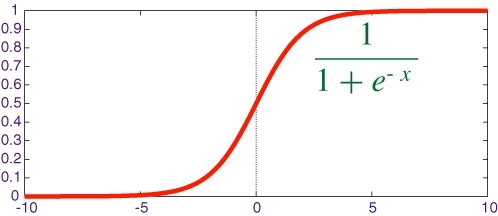
\includegraphics[width=4in]{sigmoid}
		\caption{sigmoid函数$f \left(x\right) $图像}
		\label{gra-sigmoid}
	\end{center}
\end{figure}

联系公式\eqref{eq19}与公式\eqref{pairwisepre},由图\ref{gra-sigmoid} sigmoid函数图像可得, 当$f \left(x_{uij}\right) \rightarrow +1$时, 也就是$x_{uij} = \hat{r}_{ui} - \hat{r}_{uj}$越来越大, 即用户对于物品$v_i$与$v_j$的预测差值越来越大. 因此为了加速学习, 针对一个已有的user-item pair中的物品 $v_i$,要采样的物品$v_j$应当是$v_i$相比有竞争力的物品, 更进一步说也就是由该用户对于$v_i$与$v_j$的偏好得分应该是相近的,否则这个采样对于SGD便是低效的采样。

从经验上来讲,每个用户只会浏览一小部分的物品并对这些浏览过的物品提供一些交互反馈。如果均匀采样器均等地从整个物品集合中采样negative  item.对于一个user-item  pair,大部分均匀采样的物品并不具有可比性或者很难被相关的用户浏览。举个例子,iPhone与牙刷或iPhone与一个冷门的手机品牌可能会经常被均匀采样器采得。而由于这些低效的training pair对于SGD几乎作用很小,整个训练过程便会收敛地极其缓慢。

除此以外,与经典的分解技术相似,如果一个用户或物品缺乏足够的反馈,其对应的隐式表达往往不能够被很好的学习到。在现实世界数据集中,用户行为与物品流行度的分布往往呈现长尾状。这就导致了大部分的用户和物品仅仅有很小部分的反馈数据。此外,在真实的推荐系统中,新的个体可能在任何时间被加入到推荐系统中。因此,BPR框架也很容易受制于冷启动问题。

\subsection{Latent Dirichlet Allocation}
Latent Dirichlet allocation(LDA),隐含狄利克雷分布,是一种主题模型(topic model),它可以将文档集中每篇文档的主题按照概率分布的形式给出。同时它是一种无监督学习算法,在训练时不需要手工标注的训练集,需要的仅仅是文档集以及指定主题的数量即可。此外LDA的另一个优点则是,对于每一个主题均可找出一些词语来描述它。

LDA首先由于2003年提出\cite{blei2003latent},目前在文本挖掘领域包括文本主题识别、文本分类以及文本相似度计算方面都有应用。


\subsubsection{数学模型}
LDA是一种典型的词袋(Bag-of-words)模型,即它认为一篇文档(document)是由一组词(word)构成的一个集合,词与词之间没有顺序以及先后的关系。一篇文档可以包含多个主题(topic),文档中每一个词都由其中的一个主题生成。

\begin{figure}[htbp]
	% caption放上面就会显示在图的上方,出现在下面就是出现在图的下方
	% label的位置也有讲究
	\begin{center}
		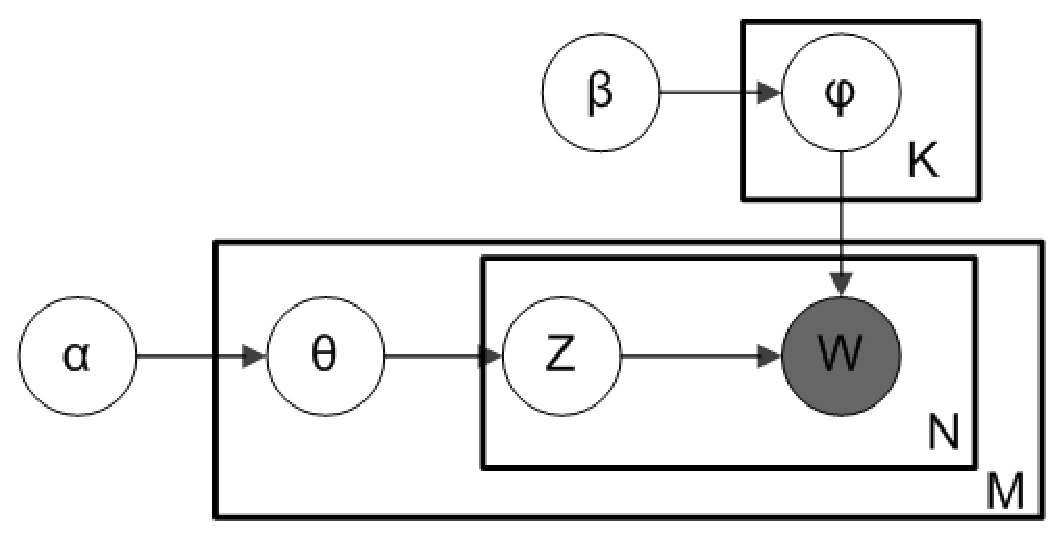
\includegraphics[width=4in]{LDA}
		\caption{LDA 贝叶斯网络结构}
		\label{gra4}
	\end{center}
\end{figure}

另外,正如Beta分布是二项式分布的共轭先验概率分布,狄利克雷分布作为多项式分布的共轭先验概率分布。因此正如图\ref{gra4}, LDA贝叶斯网络结构中所描述的,在LDA模型中一篇文档生成的方式如下:
\begin{itemize}
	\item 从狄利克雷分布$\alpha$ 中取样生成文档$i$的主题分布$\theta_i$
	\item 从主题的多项式分布$\theta_i$中取样生成文档$i$第$j$个词的主题$z_{i, j}$
	\item 从狄利克雷分布$\beta $中取样生成主题$z_{i, j}$的词语分布$\phi_{z_{i, j}}$
	\item 从词语的多项式分布$\phi_{z_{i, j}}$中采样最终生成词语$w_{i, j}$
\end{itemize}
因此整个模型中所有可见变量以及隐藏变量的联合分布是
\begin{equation}
p(w_i, z_i, \theta_i, \Phi | \alpha, \beta) = \prod_{j = 1}^{N} p(\theta_i|\alpha)p(z_{i, j}|\theta_i)p(\Phi|\beta)p(w_{i, j}|\theta_{z_{i, j}})
\end{equation}


最终一篇文档的单词分布的最大似然估计可以通过将上式的$\theta_i$以及$\Phi$进行积分和对$z_i$进行求和得到
\begin{equation}
p(w_i | \alpha, \beta)  = \int_{\theta_i}\int_{\Phi }\sum_{z_i}p(w_i, z_i, \theta_i, \Phi | \alpha, \beta) 
\end{equation}


根据$p(w_i | \alpha, \beta)$ 的最大似然估计,最终可以通过吉布斯采样等方法估计出模型中的参数。


\subsubsection{使用吉布斯采样估计LDA参数}
在LDA最初提出的时候,人们使用EM算法(Expectation-maximization algorithm)进行求解,后来人们普遍开始使用较为简单的Gibbs Sampling,具体过程如下:
\begin{itemize}
	\item 首先对所有文档中的所有词遍历一遍,为其都随机分配一个主题,即$z_{m,n}=k\sim Mult(1/K)$,其中$m$表示第$m$篇文档,$n$表示文档中的第$n$个词,$k$表示主题,$K$表示主题的总数,之后将对应的$n^{\left(k\right)}_m+1$, $n_m+1$, $n^{\left(t\right)}_k+1$, $n_k+1$, 他们分别表示在$m$文档中$k$主题出现的次数,$m$文档中主题数量的和,$k$主题对应的$t$词的次数,$k$主题对应的总词数。
	\item 之后对下述操作进行重复迭代。
	\item 对所有文档中的所有词进行遍历,假如当前文档$m$的词$t$对应主题为$k$,则$n^{\left(k\right)}_m-1$, $n_m-1$, $n^{\left(t\right)}_k-1$, $n_k-1$, 即先拿出当前词,之后根据LDA中topic sample的概率分布sample出新的主题,在对应的$n^{\left(k\right)}_m$, $n_m$, $n^{\left(t\right)}_k$, $n_k$上分别$+1$。
	\begin{equation}
	p(z_i=k|z_{-i},w) \propto k(n^{(t)}_{k,-i}+\beta_t)(n_{m,-i}^{(k)}+\alpha_k)/(\sum_{t=1}^{V}n_{k,-i}^{(t)}+\beta_t)
	\end{equation}
	\item 迭代完成后输出主题--词参数矩阵$\Phi$和文档--主题矩阵$\Theta$
	\begin{align}
	\phi_{k,t}   &=(n_k^{(t)}+\beta_t)/(n_k+\beta_t)  \\
	\theta_{m,k} &=(n_m^{(k)}+\alpha_k)/(n_m+\alpha_k)
	\end{align}
\end{itemize}









\subsection{本章小结}
本章首先介绍了采用SGD求解的Bayesian Personalized Ranking(BPR)推荐算法, 并且对可能导致其收敛缓慢的均匀采样策略做了讨论。然后简要介绍了LDA模型。
	\section{适应性采样策略}
在这一章中,我们结合了内容信息与隐式反馈提出了一个非均匀的物品采样器(a non-uniform item sampler)。在本章中所提出的适应性采样策略(adaptive sampling strategy)自动地模拟了真实的数据分布并且具有适应性地挑选更有针对性的train pairs.


\subsection{适应性采样策略概览}
在现实世界的场景中,用户常常会浏览同一个目录下的多个物品,然后做出他们的选择。那么很显然,我们应该采样具有针对性的物品,比方说针对iPhone,相对于毛巾或者某低档品牌的手机, 采样高档Samsung或者LG显然更具有可比性与合理性。

因此,在适应性采样策略中,我们倾向于采样那些对于用户已选择过的物品更具有可比性同时有很大机会被相关用户浏览的物品。更确切的说,对于一个user-item pair$\left(u_m,v_i\right)$,我们通过以下的步骤采样一个更加合理的负样本(negative item)$v_j$:
\begin{enumerate}
	\item 根据用户$u_m$与物品$v_i$的所在目录分布(categorical distribution),首先推断对于事件用户$u_m$选择物品$v_i$会发生在哪个目录下。
	\item 
	对于给定的一个目录,在该目录下我们进一步选择物品$v_j$作为negative item,而该物品同时又具有较高的概率能够被用户$u_m$所浏览。
\end{enumerate}




\subsection{类别分布}
在适应性采样中, 首先需要知道用户与物品的类别分布(categorical distribution). 不过在有些实际的应用场景中,由于缺乏类别信息,推荐系统并无法直接得到用户与物品的类别分布。为了应对这个问题,我们利用了所谓的隐式表达(the latent representation of an entity)来近似指示其类别信息。

首先我们假设一个entity可能属于多个目录 $C = \{c_1,c_2,\cdots,c_k\}$ ,并且它的类别分布服从幂率(power laws)分布\cite{rendle2014improving}. 用$y_i^e \in \mathbb{R}^k$ 表示 entity $e_i$ 的latent vector ,而矩阵 $Y_e = \left[y_1^e,y_2^e,y_3^e,\cdots\right]$ 是从内容信息(content information)与隐式反馈(implicit feedback)学习得到的entities's latent representation. 以推荐系统中的一个经典场景为例:在推荐系统有两种类型的实体(entity),也就是说用户users, 比如消费者, 和物品items, 比如说电影,书籍和歌曲等。明确起见,本论文使用上标$u$与$v$分别表示与用户user和物品item相关的变量。比如,$y^u_m$表示the latent vector of user $u_m$,$Y^u$表示the latent representation matrix of user, $y_i^v$表示the latent vector of item $v_i$.为了联系categorical distribution 与 the latent vector of entity, 我们认为 entity $e_i$属于目录$c\in C$的概率$p\left(c|e_i\right)$为标准化因子的混合(a mixture over standardized factors),并将其定义为:

\begin{equation}
p\left(c|e_i\right)  \propto exp\left( \frac {y_{i,c}^e - \mu_c}{\sigma_c} \right)
\end{equation}

这里的$\mu_c = E\left(y_{*,c}^e\right)$,$\sigma_c = Var\left(y_{*,c}^e\right)$分别表示all entity factors的经验均值与方差(empirical mean and variance over all entity factors)。假设在用户与物品上的类别分布是相互独立的,那么就可以进一步推断user-item pair$\left(u_m,v_i\right)$同属于一个category $c$的联合概率$p\left(c|u_m,v_i\right)$:

\begin{equation}
\label{eq21}
p\left(c|u_m,v_i\right) = p\left(c|u_m\right)p\left(c|v_i\right)
\end{equation}

根据其联合概率,就可以根据时间用户$u_m$选择物品$v_i$采样一个目录$c$。




\subsection{选取negative item $v_j$}
对于给定一个目录$c$,下一步的目标便是在该目录下选取一个negative item $v_j$,而$v_j$同时将有很大概率会被用户$u_m$所浏览. 

\subsubsection{物品浏览概率}
一个简单点的做法,我们可以将entity $e_i$在目录$c$下的排序得分(ranking score)视作为$p\left(c|e_i\right)$,再进一步从根据它们的排序得分直接选择物品。但实际上,浏览概率(browsing probabilities)与排序得分(ranking scores)并不等同,显然两者之间存在差距。在实际场景中,对于出现在排序列表(ranking lists)中的物品,那些排在靠前位置的物品相对于靠后位置的物品, 往往有着极大的概率被用户所浏览。比如在整个列表中排名前三位的物品的极有可能都会被用户所浏览,而他们排序得分不同的影响在这种情况下将微乎其微。为了应对这个问题,对于给定目录下的物品采样我们分为两步进行:
\begin{enumerate}
	\item 首先,我们先根据经验分布(empirical distribution)从候选物品(candidates)中采样一个排序的位置$r$;
	\item 然后,在该目录下对物品进行排序,返回在位置$r$处的物品作为我们采样的negative item。
\end{enumerate} 

典型地,经验分布大致服从analytical law, 比如Geometric\cite{wang2009pskip}或Zipf\cite{adamic2002zipf} distribution。在这里,我们应用Geometric distribution到从目录$c$的排序列表中选取位置$r(j)$处的物品$v_j$:

\begin{equation}
p\left(v_j|c\right) \propto exp\left(-r\left(j\right)/\lambda\right),\lambda \in \mathbb{R}^+
\end{equation}

这里的$r\left(j\right)$表示物品$v_j$的排序位置,$\lambda$是用来调整概率密度的超参数(hyper-parameter)。




\subsubsection{如何对物品列表进行排序}
在获得negative item的排序位置后,接下来的任务便是如何在这个位置安排对应的物品。\cite{rendle2014improving}中有一个简单的方法:将物品的 latent factors 当作其 ranking scores, 然后根据它们的排序得分(ranking scores)对物品进行排序. 但是由于物品的latent factors在每轮迭代都会被更新,这种方法不得不在每轮迭代每个目录下对物品进行重新排序。这会导致一个很高的计算复杂度,因为每轮迭代需要花费$\mathit{O}\left(kt\log t\right)$的运行时间来进行重新排序,这里的$t$指物品数。为此在\cite{rendle2014improving}中同样提出一个妥协性的做法:每迭代$t \log t$轮再进行重新排序。不过这种妥协会很容易导致局部收敛(local convergence)。此外, 每隔$t\log t$轮进行更新, 实际上在很多未更新的时候的采样相当于从一个随机的物品子集中随机采样, 此时的采样反而会产生副作用。更进一步, 由于items' latent vectors 是被随机初始化, 那么排序列表在首次重排序之前其实是相当于一个随机序列。如果这个随机的排序列表未被及时更新, 那么采样器实际上会衰退为从一个物品子集中随机采样的采样器。因此, 需要一个新的采样方法来平衡效率与推荐表现。

\begin{figure}[htbp]
	\begin{center}
		\includegraphics[width=3.5in]{subspace.png}
		\caption{将不同模态(different modalities)的entity映射到一个共享的隐式空间(a shared latent space). 在这里假设协同信息(collaborative information), 比如评分(rating), 和内容信息(content information), 比如文本(text),分属于不同模态,正如图中的space A, space B.}
		\label{gra5}
	\end{center}
\end{figure}

根据对于子空间的研究\cite{udupa2010improving,rasiwasia2010new},如果我们将一个entity从不同模态的映射到一个共享子空间,那么它在子空间中的表达应当是具有关联性的,比如互补(complementary)或是相似(similar)。如果我们独立地将一个item从content space和collaborative space映射到a shared latent space,那么我们就能够得到一个item在共享隐式空间的两个latent representations.如图\ref{gra3}所示. 为了避免采样器衰退为从一个物品子集中随机采样一个物品, 我们通过物品的协同信息(collaborative filtering)来初始化排序列表(ranking lists)。具体来说, 我们首先通过特征学习(feature learning)的方法从协同信息中学习物品的一个近似的隐式表达(latent representation), 比如, 用于图像的Conventional Neural Networks(CNN), 用于文本的Latent Dirichlet Allocation(LDA)。那么, 我们将latent factors视作为在目录分布下的物品排序得分, 然后在每个目录下对物品进行排序. 最终, 我们就根据这些排序后的结果对物品排序列表进行初始化。

此外, 为了避免局部收敛的问题, 同时平衡效率, 我们\textbf{只对于那些热门目录下的物品进行重排序}。根据公式\eqref{eq21}, 首先对于一个user-item pair选定一个目录, 然后进一步计算在每个目录下出现了多少所观测的user-item pairs.定义变量$\rho \in \mathbb{R}^k$来表示目录的热度(popularity of categories)。在每次迭代中, 我们根据目录的热度采样出一个热门目录(popular category) $c$:
\begin{equation}
p\left(c|p\right) \propto exp\left(\frac{\rho_c - \mu }{\sigma}\right)
\end{equation}
这里的$\mu$ 和$\sigma$分别表示$\rho$的经验均值与方差(empirical mean and variance). 然后, 我们将物品的current latent factors视为物品的new ranking scores, 并衡量在目录$c$下的new score vector, 根据a similarity function $sim\left(\cdot,\cdot\right)$与旧的score vector相比是否有较大变化.如果ranking score vector的变化超过了阈值 $\delta$, 就用物品的latent represenration matrix 的第$c$列$y_{*,c}^v$来更新在目录$c$下的ranking scores, 并且对该目录下的物品进行重新排序.

\subsection{适应性采样算法}


总言之,在本论文中所研究的适应性采样策略如算法$\ref{al2}$所示, 对于一个user-item pair$\left(u_m,v_i\right)$, 采样一个negative item $v_j$, 而$v_j$与$v_i$相比, 不仅具有可比性,而且具有较高的几率为用户所浏览。在算法$\ref{al2}$中, $index\left(c,r\right)$返回在排序列表$l_c \in L$中位置在$r$处的物品。$x_c \in X$是在目录$c$下的ranking score vector, 而$x_c$正是由从协同信息学习而来approximate latent representation所初始化。值得注意的是, 在整个学习过程中,本论文的适应性采样策略仅需要在一些热门目录重排序几次, 这不仅降低了计算复杂度同时避免了局部极值(local extremum)。

\IncMargin{1em}
\begin{algorithm}
	\SetAlgoNoLine %不要算法中的竖线
	
	\SetKwInOut{Input}{\textbf{输入}}\SetKwInOut{Output}{\textbf{输出}}
	
	\Input{
		\\
		The observed user-item pair set $\mathcal{P}$\;\\
		The counters of category popularity $\rho$\;\\
		The latent representation matrixes $Y^u$ and $Y^v$\;\\
		The ranking scores of items $X = \{x_1,x_2,\cdots,x_k\}$\;\\
		The orders of items $L = \{l_1,l_2,\cdot,l_k\}$\;\\}
	\Output{
		\\
		The training triple $\left(u_m,v_i,v_j\right)$\;\\
		The category popularity $\rho$\;\\
		Draw a category from $p\left(c|\rho\right)$\;\\}
	\BlankLine
	 Draw a popular category $c$ from $p\left(c|\rho\right)$\;
	 \If {$sim \left(x_c,y_{*,c}^v\right) > \delta $}{
		 Update $x_c$ by $y_{*,c}^v$\;
		 Reorder items under $c$ and update $l_c$\;
	 }
	 Draw $\left(u_m,v_i\right) \in \mathcal{P}$ uniformly\;
	 Draw a category $c$ from $p\left(c|u_m,v_i\right)$,$\left(1\leq c \leq k\right)$\;
	 $\rho_c ++$\;
	 Draw a rank $r$ from $p\left(r\right) \propto exp\left(-r/\lambda\right),\left(1\leq c \leq k\right)$\;
	  
	 $v_j \leftarrow 
	 \begin{cases}
	 index\left(c,r\right) & if \ sgn\left(y_{m,c}^u\right) = 1\\
	 index\left(c,n-r-1\right) & else
	 \end{cases}$\;
	 
	\caption{Content-aware and Adaptive sampling}
	\label{al2}
\end{algorithm}
\DecMargin{1em}




\subsection{本章小结}
本章主要介绍了适应性采样策略, 该采样策略通过采样一个具有可比性同时又有较大概率被用户浏览的物品作为negative item。该采样策略不仅能够降低计算复杂度同时能够避免局部极值。
	\section{融合内容信息的适应性BPR}
在上述章节中, 我们阐述了如何通过一个适应性采样策略加快BPR的学习, 同时通过仅考虑隐式反馈学习了the latent factors of entities。 不过, 在现实世界的推荐系统中, 很可能没有足够的协同信息, 比如, 新的物品可能会在任何时间被加入到推荐系统中。因此, 我们提出一个更为全面的个性化推荐方法:Content-aware and Adaptive Bayesian Personalized Ranking, 它基于上面所提出的适应性采样策略, 同时将隐式反馈与内容信息融合入一个统一的推荐框架中.


\subsection{Learning Content-aware Mappings}
我们首先正提出一个对于学习content-aware mappings的一个非监督解决方案。用矩阵$A^e = \left[a_1^e,a_2^e,a_3^e,\dots\right]$来表示content features of entities.然后我们提出对于学习content-aware mappings的目标函数:
\begin{equation}
L_{content} = \| A^eW^e - Y^e\|_F^2
\end{equation}
这里的$W^e \in \mathbb{R}^{d^e \times k}$表示映射矩阵(mapping matrix), $k$表示latent vectors的维度。




\subsection{Parameter Inference of CA-BPR}
通常来讲, 由于缺乏监督信息(supervised information),在公式所表述的优化问题并无确定解法。不过, 根据子空间的研究, 我们可以从隐式反馈中学习一个latent matrix $\widetilde{Y^e}$, 并用$\widetilde{Y^e}$近似代替$Y^e$. 因此, 将$\widetilde{Y^e}$代替$Y^e$代入公式, 那么目标函数变为: 
\begin{equation}
L_{content} = \| A^eW^e - \widetilde{Y^e}\|_F^2
\end{equation}

使用$\widetilde{Y^e}$近似代替$Y^e$不仅能够优化目标函数, 同时还能够一起学习包含协同信息与内容信息的 $W^{e}$. 因此, 算法总体的目标函数如下:
\begin{equation}
%分隔一个过长的公式分行显示使用split环境
\begin{split}
arg \min_{\substack{\Theta, W}} L_{feedback}+L_{content}  = 
& - \sum_{\left(m,i,j\right) \in D_s} \ln f \left( r_{mij}\right) + \lambda\|\theta\|^2\\
& + \|A^eW^e-Y^e\|^2_F + \frac 12 \sum_{e\in \{u,v\}}\lambda^e\|W^e\|^2_F 
\end{split}
\end{equation}
这里的$r_{mij} = r_{mi} -r_{mj}$。
为了学习在公式中的参数$Y^u$, $Y^v$, $W^u$, $W^v$, 在每轮迭代中, 当我们更新latent factor matrix $Y^e$, 将矩阵$W^e$认为是一个常量(constant), 并将$L_{content}$视作一个正则化项(regularizer)。那么, 对于一个任意 latent parameter $\theta$ 的梯度如下:
\begin{equation}
\begin{split}
\frac{\partial L}{\partial\theta} = 
& \sum_{\left(m,i,j\right) \in D_s}\left(f\left(r_{mij}\right) - 1\right) 
\frac{\partial \left(r_{mij}\right)}{\partial \theta}\\
& + \frac{\partial \sum_{e \in \{u,v\} } \lambda^e \left(\|A^eW^e-Y^e\|_F^2\right)}{\partial \theta}   + \lambda \theta 
\end{split}
\end{equation}
对于参数$\theta$的更新公式为: $\theta = \theta - \gamma \frac{\partial L}{\partial \theta}$, 这里的$\gamma$为学习率(learning rate)。另一方面, 对于一个latent factor matrix $Y^e$, 将$Y^e$视为伪标签(pseudo labels), 并视$L_{feedback}$为常量。因此对目标求偏导:
\begin{equation}
\frac{\partial L}{\partial W^e} = \left(A^e\right)^T\left(A^eW^e-Y^e\right) + \lambda^e W^e
\end{equation} 
令$\frac{\partial L}{\partial W^e} = 0$, 那么对于$W^e$的更新公式则演变为:
\begin{equation}
\label{equ:W}
W^e = \left(\left(A^e\right)^TA^e + \lambda^e\mathbb{E}\right)A^eY^e
\end{equation}
这里的$\mathbb{E} \in \mathbb{R}^{k\times k}$表示一个单位矩阵。

总言之, 对于CA-BPR的参数学习如算法2所示.
\IncMargin{1em}
\begin{algorithm}
	\SetAlgoNoLine %不要算法中的竖线
	
	\SetKwInOut{Input}{\textbf{输入}}\SetKwInOut{Output}{\textbf{输出}}
	
	\Input{
		\\
		The observed user-item pair set $S$\;\\
		The feature matrix of items $F$\;\\
		The content features entities $A := \{A^u,A^v\}$\;\\}
	\Output{
		\\
		$\Theta \  := \{Y^u,Y^v\}$\;\\
		$W := \{W^u,W^v\}$\;\\}
	\BlankLine
	initialize the model parameter $\Theta$ and $W$ with uniform $\left(-\sqrt{6}/{k},\sqrt{6}/{k}\right)$\;
	standarized $\Theta$\;
	Initialize the popularity of categories $\rho$ randomly\;
	\Repeat
		{\text{convergence}}
		{Draw a triple $\left(m,i,j\right)$ with 算法\ref{al2}\;
			\For {each latent vector $\theta \in \Theta$}{
				$\theta \leftarrow \theta - \eta\frac{\partial L}{\partial \theta}$
			}
			
			\For {each $W^e \in W$}{
				Update $W^e$ with the rule defined in Eq.\ref{equ:W}\;
			}	
		}
		
		
	\caption{Learning paramters for BPR\label{al3}}
	
\end{algorithm}
\DecMargin{1em}

\subsection{本章小结}
本章通过学习了一个mapping矩阵利用了内容信息,同时将本文所研究的适应性采样策略融合BPR的推荐框架中,提出了CA-BPR推荐算法。
	\section{结论与展望}
\subsection{结论}
智能网联汽车由于其大量集成了各类先进技术,复杂性相较于传统汽车有很大的提高。也正因如此,智能网联汽车比起传统汽车有可能会面临到更多的安全风险。本文关注智能网联汽车在GNSS位置攻击欺骗方面的检测算法工作,并在实验中成功验证了所设计的检测算法的有效性。更进一步地,本文还基于ISO 26262标准,对智能网联汽车在受到GNSS位置欺骗攻击后可能面临的功能安全风险进行了分析,并提出了相应的应急策略,从而实现检测算法与应急策略的联动。
\subsection{进一步研究工作}
尽管本文在实验中验证了所设计的检测算法可以有效完成检测工作,但是并没有将不同场景下GNSS定位的精确度纳入考虑。具体而言,欺骗阈值$\gamma$应该在不同的场景下,如城市高楼间、平原、隧道内、地下停车场等,具有一定不同的值。但由于目前缺少各种场景中GNSS定位精确度的相关数据,这项工作暂时无法进行。下一步将考虑在实车上采集数据,从而完善检测算法在不同场景下的表现。

	\section{结论与展望}

\subsection{本文的主要内容}

本文首先回顾了采用均匀采样策略的经典BPR推荐算法,然后分析其在随机梯度学习算法中导致收敛缓慢的原因。而后在隐式反馈的基础上加入内容信息提出了非均匀的适应性采样策略,并将其融入BPR推荐框架中。实验证明本文所研究的方法的确能够提高推荐效果。

\subsection{进一步的研究工作}
尽管本文实验证明通过加入内容信息的确有助于提高推荐效果,但是对于加入内容信息的适应性采样策略在整个学习过程每个阶段的影响仍然有待研究。同时对于一些已有的一些融合内容信息的推荐方法,比如采用Word2Vec技术,还需进一步的研究调查在这些融合内容信息的不同推荐方法中的特点,适用性及其局限性。


	%参考文献
	\kaishu
	\bibliographystyle{plain}
	\addcontentsline{toc}{section}{参考文献} %向目录中添加条目,以章/section的名义
	\bibliography{main}


	%致谢与英文摘要
	\fangsong
	\newpage

\section*{\centerline{\heiti\zihao{-4}{致谢}}}
\addcontentsline{toc}{section}{致谢}

首先衷心地感谢潘微科老师。在本科生涯最后的一年多里,不仅是现时的学业与学术, 更是对于未来的发展给予了我很多指导与帮助。本次毕业设计,从选题到论文撰写,给予了我很多宝贵的意见。他渊博的学识、严谨的治学态度及认真负责的工作态度都使我受到鼓舞和熏陶。在此向潘微科老师表示崇高的敬意和衷心的感谢, 他的言传身教将使我终生受益。

\vspace{5bp}
感谢key哥哥与在453认识的朋友们, 与你们的交流大概就是我对计算机启蒙的开始. 如果不是有幸与你们相识, 这一路走来必是要曲折地多.

\vspace{5bp}
感谢 Thuthesis 及其作者薛瑞尼. 最终虽未使用Thuthesis模板, 但是此间对其研习所得对我顺利使用 \LaTeX 完成论文撰写仍然起了很大作用.

\vspace{5bp}
感谢一直关心我的父母与兄长。远游在外, 感谢还有你们牵挂.

\vspace{5bp}
感谢自己熬过了那段难捱的日子。从学习画画到广播电视再到计算机科学, 在如今看来似曾是做了诸多无用功, 不过幸而没有因为短时的平庸迷茫而消磨掉满心的戾气. 

\vspace{5bp}
前路漫漫, 不冀求大步流星, 唯盼能步步坚实.
	\newpage

\centerline{\fangsong\bf\zihao{-2}{Research on Content-Aware Collaborative Filtering }}

\addcontentsline{toc}{section}{Abstract(Key words)}

\vskip 20bp

\hspace{4bp} {\zihao{-4}\textbf{【 Abstract】}}
With the booming development of machine learning, data mining and other technologies, various emerging technologies are being created. This includes intelligent connected cars. Smart Internet-connected vehicles are different from traditional cars in that they are equipped with various sensors and actuators, as well as combined with modern communication and interconnection technologies, which can realize information exchange between vehicles, vehicles and people, and vehicles and roads. However, the GNSS location spoofing problem associated with intelligent connected cars also frequently plagues major manufacturers and researchers. Therefore, this paper focuses on the detection of GNSS position spoofing attacks on intelligent connected cars and the corresponding functional safety contingency strategies. The main work of this paper can be summarized as the following three points.
\begin{enumerate}
    \item For GNSS position spoofing attacks on intelligent connected cars, an algorithm that can effectively implement attack detection is designed and implemented based on LSTM networks in machine learning, using publicly available datasets to build a training set. The data needed to train the LSTM network are velocity, steering angle, forward acceleration, and the distance the vehicle moves between adjacent time stamps. In this paper, the GNSS location point data in the original data are converted into distances by using the Haverson's great circle formula.
    \item The spoofing dataset was obtained by modifying part of the data in the public dataset, and experiments were conducted with this as the test set. The experimental results show that the algorithm designed in this paper can effectively detect GNSS location spoofing attacks against intelligent connected cars.
    \item Based on the ISO 26262 standard, the functional safety risks that intelligent connected vehicles may face in the case of GNSS location spoofing attacks are analyzed using the HARA method, and the corresponding risk levels are also classified, and suitable contingency strategies are designed. Thus, the linkage of algorithm detection and contingency strategy is realized.
\end{enumerate}
In summary, this paper designs a location spoofing attack detection algorithm based on LSTM technology and ISO 26262 standard for the GNSS module of intelligent connected cars, and also designs a corresponding functional safety contingency strategy. The detection algorithm can work effectively, but there is still room for improvement in the scene refinement. The GNSS positioning error in different scenarios can be obtained later by collecting data from real vehicles, so as to refine the detection performance in different driving scenarios.

\vskip 10bp

\hspace{5bp}{\zihao{-4}\textbf{【 Keywords】}}
intelligent Connected Vehicle; GNSS; Functional Safety; LSTM


\vskip 20bp

\begin{flushright}
	\kaishu 指导教师:\ 肖志娇 \hspace{3cm}{ }
\end{flushright}

\label{lastpage}%%%%显示总页数

\end{document}
